\documentclass[hidelinks, 12pt]{article}
\usepackage[italian]{babel}
\usepackage{natbib}
\usepackage{url}
\usepackage[utf8x]{inputenc}
\usepackage{amsmath}
\usepackage{graphicx}
\graphicspath{{images/}}
\usepackage{parskip}
\usepackage{fancyhdr}
\usepackage{vmargin}
\usepackage{float}
\usepackage{hyperref}
\setmarginsrb{3 cm}{2.5 cm}{3 cm}{2.5 cm}{1 cm}{1.5 cm}{1 cm}{1.5 cm}

\title{Predicting soccer results}				% Title
\author{Basso Matteo \\ Ferri Marco}								% Author
\date{Giugno 2019}				% Date

\makeatletter
\let\thetitle\@title
\let\theauthor\@author
\let\thedate\@date
\makeatother

\pagestyle{fancy}
\fancyhf{}
\rhead{Basso M., Ferri M.}
\lhead{\thetitle}
\cfoot{\thepage}

\begin{document}
	
%%%%%%%%%%%%%%%%%%%%%%%%%%%%%%%%%%%%%%%%%%%%%%%%%%%%%%%%%%%%%%%%%%%%%%%%%%%%%%%%%%%%%%%%%

\begin{titlepage}
	\centering
	\vspace*{0.5 cm}
	
\includegraphics[scale = 0.75]{images/LogoBicocca.pdf}\\[1.0 cm]	% University Logo
	\textsc{\LARGE Università degli studi di}\\[0.2 cm]
	\textsc{\LARGE Milano-Bicocca}\\[2.0 cm]	% University Name
	\textsc{\Large F1801Q127}\\[0.5 cm]				% Course Code
	\textsc{\large Modelli probabilistici per le decisioni}				% Course Name
	\rule{\linewidth}{0.2 mm} \\[0.4 cm]
	{ \huge \bfseries \thetitle}\\
	\rule{\linewidth}{0.2 mm} \\[1.5 cm]
	
	\begin{minipage}{0.4\textwidth}
		\begin{flushleft} \large
			\emph{Studenti:}\\
			\theauthor
		\end{flushleft}
	\end{minipage}~
	\begin{minipage}{0.4\textwidth}
		\begin{flushright} \large
			\emph{Matricole:} \\
			807628 \\ 807130
		\end{flushright}
	\end{minipage}\\[2 cm]
	
	{\large \thedate}\\[2 cm]
	
	\vfill
	
\end{titlepage}

%%%%%%%%%%%%%%%%%%%%%%%%%%%%%%%%%%%%%%%%%%%%%%%%%%%%%%%%%%%%%%%%%%%%%%%%%%%%%%%%%%%%%%%%%

\tableofcontents
\pagebreak

%%%%%%%%%%%%%%%%%%%%%%%%%%%%%%%%%%%%%%%%%%%%%%%%%%%%%%%%%%%%%%%%%%%%%%%%%%%%%%%%%%%%%%%%%



\section{Abstract}

Il calcio è da anni lo sport più giocato e diffuso in svariati paesi del mondo. Moltissime persone seguono settimanalmente, con grande attenzione e fervore, ogni singola partita nella speranza di veder vincere la propria squadra del cuore.

In questo contesto si sono inevitabilmente sviluppati un gran numero di diversi business di enorme valore economico, fra cui ad esempio quello delle scommesse. Saper prevedere l'esito di una partita, sia in termini di vittoria che di goal fatti, rappresenta per moltissimi un argomento di particolare interesse. Durante questo studio, ci si è posti l'obiettivo di sviluppare un modello per la predizione del risultato delle partite di calcio in maniera automatica. Tale predizione deve essere basata sulla formazione delle due squadre considerate per ciascuna partita, nonché sulle caratteristiche dei giocatori coinvolti.

Il dominio di riferimento è stato modellato attraverso l'utilizzo di una Rete Bayesiana attraverso la quale fare le dovute inferenze e conseguentemente predire il risultato di una partita fra due squadre di calcio. Il medesimo approccio potrebbe essere riutilizzato in altri sport o giochi che prevedano l'interazione fra più squadre di cui si conoscono le statistiche di ciascun giocatore.



\clearpage



\section{Introduzione}

Viene qui presentata una visione generale del progetto, ovvero il dominio di riferimento e gli obiettivi che esso si pone, le scelte di design per la creazione del dataset ed eventuali ipotesi o assunzioni fatte durante lo sviluppo dell'elaborato.



\subsection{Dominio di riferimento}

Il calcio rappresenta, soprattutto negli ultimi anni, lo sport maggiormente diffuso in vari paesi del mondo. Molte persone seguono con grande attenzione tutte le partite cercando di capire preventivamente il vincitore, per piacere personale oppure per giocare nel mercato delle scommesse.

A seguito di questo fenomeno sono stati creati svariati portali che permettessero alle persone di entrare sempre di più in questo mondo. Un aspetto fondamentale per ogni piattaforma di scommesse è senz'altro la possibilità di predire il vincitore di un match attraverso la simulazione di partite di calcio con particolari formazioni.



\subsection{Obiettivi dell'elaborato}

Questo elaborato sarà suddiviso per argomenti, secondo un approccio di indagine incrementale e coerente con quanto praticamente svolto.

Verranno innanzitutto descritte le modalità di acquisizione dei dati dalla sorgente, a cui sarà associata anche una breve descrizione di quanto a disposizione. Quindi, si esploreranno i criteri e le assunzioni che hanno portato alla creazione del dataset su cui sviluppare il modello di predizione. Con questo, si intende dire che verranno inizialmente presentate alcune analisi qualitative sui dati e successivamente descritti i procedimenti svolti per l'integrazione e l'estrazione delle informazioni più rilevanti.

In seguito all'esportazione del dataset saranno descritte le modalità di suddivisione del dataset su cui fare inferenze, in particolare attraverso l'utilizzo delle Reti Bayesiane. Diversi modelli di generazione della rete verranno presentati e per ognuno saranno analizzati i risultati ed evidenziate le differenze. L'obiettivo del modello è quello di predire il team vincitore di un determinato match, utilizzando le informazioni dei giocatori presenti in campo.

Verrà infine presentata un'interfaccia utente per la simulazione di una partita di calcio, utile a mostrare l'effettivo impiego della rete in un prodotto di natura commerciale e pensato per l'utilizzo sul Web.



\clearpage



\section{Descrizione del dataset originale}

Di seguito viene presentata la descrizione del dataset originale, prelevato da Kaggle \cite{site:kaggle-dataset} e a sua volta creato attraverso l'unione di dati provenienti da diverse fonti, fra cui la più importante contenente le statistiche del famoso videogioco di calcio EA Sports FIFA. \cite{site:ea-fifa}. Il contenuto del dataset è rappresentato dalle principali squadre e giocatori di calcio in Europa, con le partite svolte in un periodo temporale di 6 anni.



\subsection{Formato}

Il dataset consiste di un database SQLite \cite{site:sqlite}, ovvero un file con omonima estensione contenente un database relazionale di rapido utilizzo, in grado di essere condiviso e utilizzato facilmente su un qualsiasi dispositivo.



\subsection{Giocatori}

I giocatori sono espressi all'interno di due tabelle differenti nello schema del database considerato. La prima relazione denominata {\it Player} contiene informazioni di carattere generale ed è mostrata in tabella \ref{tab:player} a seguire.

\begin{table}[H]
	\caption{Player}\label{tab:player}
	\centering
	\begin{tabular}{|l|l|l|}
		\hline
		Campo & Descrizione \\
		\hline
		id & Id del record \\
		player\_api\_id & Identificativo univoco del giocatore \\
		player\_name & Nome completo del giocatore \\
		player\_fifa\_api\_id & Id utile per reperire le informazioni da fifa \\
		birthday & Data di nascita \\
		height & Altezza in centimetri \\
		weight & Peso in libbre \\
		\hline
	\end{tabular}
\end{table}

La seconda tabella, denominata {\it PlayerAttributes} contiene invece i punteggi associati alle abilità personali di ciascun giocatore. Essa contiene inoltre un campo che indica a quale data tali punteggi si riferiscono, cioè quando sono state effettuate le rilevazioni. É possibile, infatti, che i dati associati ad un giocatore cambino nel tempo; per tale motivo, nel momento in cui si rivelerà necessario recuperare i dati dei giocatori facenti partecipanti ad una partita, sarà necessario selezionare i giusti record dalla tabella \textit{Player} proprio in base alla data della partita.

Nella tabella \ref{tab:player_attr} vengono meglio elencati i campi che descrivono un giocatore. La maggior parte di essi sono espressi su una scala intera da 1 a 100.

\begin{table}[H]
	\caption{PlayerAttributes}\label{tab:player_attr}
	\centering
	\begin{tabular}{|l|l|l|}
		\hline
		Campo & Descrizione \\
		\hline
		id & Id del record \\
		player\_api\_id & Identificativo univoco del giocatore \\
		player\_fifa\_api\_id & Id utile per reperire le informazioni da FIFA \\
		date & Data di riferimento del record \\
		overall\_rating & Valutazione generale \\
		potential & Potenziale \\
		preferred\_foot & Piede preferito \\
		attacking\_work\_rate & Punteggio di attacco \\
		defensive\_work\_rate & Punteggio di difesa \\
		crossing & Cross \\
		finishing & Capacità di finalizzare (segnare un goal) \\
		heading\_accuracy & Tiro di testa \\
		short\_passing & Passaggio corto \\
		volleys & Tiro al volo \\
		dribbling & Dribbling \\
		curve & Tiro con effetto curvilineo \\
		free\_kick\_accuracy & Accuratezza dei calci piazzati \\
		long\_passing & Passaggio lungo \\
		ball\_control & Controllo di palla \\
		acceleration & Accelerazione \\
		sprint\_speed & Velocità in scatto \\
		agility & Agilità \\
		reactions & Reattività \\
		balance & Equilibrio \\
		shot\_power & Potenza di tiro \\
		jumping & Salto \\
		stamina & Resistenza \\
		strength & Forza \\
		long\_shots & Tiri lunghi \\
		aggression & Aggressività \\
		interceptions & Intercettazione \\
		positioning & Posizionamento \\
		vision & Vista \\
		penalties & Falli commessi \\
		marking & Capacità di marcare \\
		standing\_tackle & Contrasto in piedi \\
		sliding\_tackle & Scivolata \\
		gk\_diving & Tuffo (portiere) \\
		gk\_handling & Presa (portiere) \\
		gk\_kicking & Rinvio (portiere) \\
		gk\_positioning & Posizionamento (portiere) \\
		gk\_reflexes & Riflessi (portiere) \\
		\hline
	\end{tabular}
\end{table}



\subsection{Squadre}

Le squadre sono descritte analogamente ai giocatori tramite 2 tabelle, {\it Team} \ref{tab:team} e {\it TeamAttributes} \ref{tab:team_attr} riportate qui di seguito.

\begin{table}[H]
	\caption{TeamAttributes}\label{tab:team_attr}
	\begin{tabular}{|l|l|l|}
		\hline
		Campo & Descrizione \\
		\hline
		id & Id del record \\
		team\_api\_id & Identificativo univoco della sqaudra \\
		team\_fifa\_api\_id & Id utile per reperire le informazioni da FIFA \\
		team\_name & Nome completo della squadra \\
		date & Data di riferimento del record \\
		buildUpPlaySpeed & Velocità di gioco \\
		buildUpPlaySpeedClass & Discretizzazione velocità di gioco \\
		buildUpPlayDribbling & Dribbling \\
		buildUpPlayDribblingClass & Discretizzazione dribbling \\
		buildUpPlayPassing & Passaggio \\
		buildUpPlayPassingClass & Discretizzazione passaggio \\
		buildUpPlayPositioningClass & Posizionamento della squadra, definito o libero \\
		chanceCreationPassing & Creazione chance di passaggio \\
		chanceCreationPassingClass & Discretizzazione creazione chance di passaggio \\
		chanceCreationCrossing & Creazione chance di cross \\
		chanceCreationCrossingClass & Discretizzazione creazione chance di cross \\
		chanceCreationShooting & Creazione chance di tiro in porta \\
		chanceCreationShootingClass & Discretizzazione creazione chance di tiro in porta \\
		chanceCreationPositioningClass & Creazione chance di posizionamento \\
		defencePressure & Pressing della difesa \\
		defencePressureClass & Discretizzazione pressing della difesa \\
		defenceAggression & Aggressività della difesa  \\
		defenceAggressionClass & Discretizzazione aggressività della difesa \\
		defenceTeamWidth & Copertura della difesa \\
		defenceTeamWidthClass & Discretizzazione copertura della difesa \\
		defenceDefenderLineClass & Tipologia di difesa \\
		\hline
	\end{tabular}
\end{table}

Come osservabile, a differenza di quanto avvenga con i giocatori, per le squadre molti attributi appaiono già discretizzati attraverso una suddivisione in classi che descrive a parole la relativa scala da 1 a 100 di ciascun campo.

\begin{table}[H]
	\caption{Team}\label{tab:team}
	\centering
	\begin{tabular}{|l|l|l|}
		\hline
		Campo & Descrizione \\
		\hline
		id & Id del record \\
		team\_api\_id & Identificativo univoco della sqaudra \\
		team\_name & Nome completo della squadra \\
		team\_fifa\_api\_id & Id utile per reperire le informazioni da fifa \\
		team\_short\_name & Nome abbreviato della squadra \\
		team\_long\_name & Nome completo della squadra \\
		\hline
	\end{tabular}
\end{table}



\subsection{Partite}

La tabella {\it Match} contiene tutte le informazioni relative alle squadre che hanno giocato una partita l'una contro l'altra, i giocatori coinvolti e il loro posizionamento in campo. I giocatori vengono numerati da 1 a 11 e il portiere viene sempre collocato in posizione [1,1]. Sono presenti inoltre dei valori il cui scopo è quello di indicare alcune specifiche tecniche sull'andamento della partita. Per brevità e mancanza di documentazione verranno semplicemente omessi, poiché poco rilevanti ai fini dello studio. Nella tabella \ref{tab:match} è presentata la descrizione dei vari campi. 

\begin{table}[H]
	\caption{Match}\label{tab:match}
	\centering
	\begin{tabular}{|l|l|l|}
		\hline
		Campo & Descrizione \\
		\hline
		id & Id del record \\
		country\_id & Id della nazione di riferimento \\
		league\_id & Id della lega di riferimento \\
		season & Stagione calcistica \\
		date & Data della partita \\
		match\_api\_id & Id univoco della partita \\
		home\_team\_api\_id & Id del team in casa \\
		away\_team\_api\_id & Id del team in trasferta \\
		home\_team\_goal & Goal del team in casa \\
		away\_team\_goal & Goal del team in trasferta \\
		home\_player\_i & Id dell'i-esimo giocatore in casa \\
		away\_player\_i & Id dell'i-esimo giocatore in traferta \\
		home\_player\_Xi & Posizione i-esimo gioc. (casa) sul lato corto del campo \\
		home\_player\_Yi & Posizione i-esimo gioc. (casa) sul lato lungo del campo \\
		away\_player\_Xi & Posizione i-esimo gioc. (trasferta) sul lato corto del campo \\
		away\_player\_Yi & Posizione i-esimo gioc. (trasferta) sul lato lungo del campo \\
		\hline
	\end{tabular}
\end{table}



\subsection{Qualche numero}
\label{sec:dataset-numbers}

Di seguito sono riportati i numeri costituenti il dataset d'origine:

\begin{itemize}
	\item 25979 partite svoltesi fra il 2010 e il 2016;
	\item 11060 giocatori in totale;
	\item 183978 rilevazioni sulle abilità dei giocatori \\ ciò significa approssimativamente 16 rilevazioni per ciascun giocatore;
	\item 299 squadre di 11 diversi campionati Europei
	\item 1458 rilevazioni sulle caratteristiche delle squadre \\ ciò significa approssimativamente 5 per ciascun squadra.
\end{itemize}




\clearpage



\section{Creazione del dataset per le predizioni}

Affinché i dati a disposizione possano essere utilizzati per la predizione del risultato di una partita su base statistica, è necessario che essi vengano prima elaborati secondo un insieme di regole su cui costruire i principi per portare a termine una specifica predizione. L'elaborazione stessa è perciò determinata sia attraverso delle assunzioni volte a identificare gli elementi più rilevanti nei dati, sia tramite l'effettiva esecuzione delle operazioni necessarie a trasformare il dataset originale in quello utilizzato per modellare la Rete Bayesiana.



\subsection{Ipotesi e assunzioni}
\label{sec:dataset-hypotesis}

Al fine di sviluppare il progetto e procedere con la stesura del seguente elaborato, sono state fatte delle assunzioni che fungono da base portante.

Si assume che il risultato di una partita, a sua volta determinato dal numero di goal segnati da una squadra e dall'altra, sia influenzato dalla bravura dei giocatori che partecipano alla partita stessa. Nel gioco del calcio, come in molti altri, esiste una netta suddivisione fra i compiti assegnati a ciascun giocatore che vanno a determinare il ruolo di quest'ultimo: \textbf{portiere}, \textbf{difensore}, \textbf{centrocampista} e \textbf{attaccante}. É chiaro che ogni ruolo riveste la sua particolare importanza e influisce in maniera diversa sull'esito della partita. Per questo progetto, si è pensato di costruire un modello basato proprio sulle potenzialità delle due squadre sfidanti nei diversi ruoli assunti dai giocatori. Poiché tale informazione è mancante all'interno del dataset originale, il primo step cui si è fatto fronte è stata la determinazione dei ruoli di ciascun giocatore in campo. Tale obiettivo è stato raggiunto attraverso l'ipotesi, più che ragionevole, secondo la quale la posizione di una persona sul campo da gioco determina anche il suo ruolo all'interno della squadra e della partita.

In secondo luogo, si è scelto inoltre di supporre che le caratteristiche del team siano determinate solo dai giocatori che ne fanno parte. Non avendo a disposizione informazioni circa l'appartenenza di un giocatore ad un determinato team nel tempo, non è possibile ottenere una suddivisione dei giocatori in squadre ben formate. Nonostante quest'ultime si potrebbero ricavare direttamente dalle partite svolte, ciò comporterebbe la creazione di dati incoerenti col mondo reale poiché i giocatori di calcio sono soggetti ad un mercato di compra-vendita su base annuale. \\
Per questo motivo, ai fini della predizione si è scelto di fatto di ignorare l'identità delle due squadre coinvolte in un match, ma semplicemente \textbf{limitarsi a considerare i 22 giocatori che hanno preso parte alla partita}, pesando adeguatamente le abilità che li contraddistinguono nel proprio ruolo.



\subsection{Scelta del formato CSV}

Per la creazione del dataset finale, utile per la modellazione della Rete Bayesiana, è stato scelto di trasformare il dataset in formato CSV, in quanto più semplice e pratico da utilizzare rispetto al database relazionale inizialmente fornito. Come si accennava, affinché possa essere creato il modello e su questo condotto delle previsioni, è necessario che i dati vengano elaborati e aggregati in un'unica tabella. Mentre SQLite consente agevolmente di lavorare sulle tabelle per effettuare \textit{join}, selezioni e proiezioni sul modello relazionale, il DBMS non è particolarmente comodo per conservare i dati una volta terminata l'aggregazione. A tale scopo si è preferito quindi esportare successivamente il risultato ottenuto all'interno di un file CSV, decisamente più portabile e immediatamente leggibile rispetto ad un database.



\subsection{Elaborazione dei dati}
\label{sec:dataset-elab}

Avendo come principale fonte d'informazione i dati relativi alle partite calcistiche svoltesi in Europa fra il 2010 e il 2016, e sapendo per ciascuna di essa i giocatori partecipanti (con relative posizioni in campo) e l'esito del match, è chiaro che la priorità durante la fase di elaborazione dei dati è stata quella di unire tutte le informazioni a disposizione in un'unica tabella. Ciò è stato possibile attraverso il \textit{join} delle tabelle \textit{Match} e \textit{PlayerAttributes} utilizzando le chiavi che le mettono in relazione. Successivamente, i dati sono stati aggregati per computare la competitività di una certa squadra in una specifica partita.


\subsubsection{Reperimento delle informazioni sui giocatori di una partita}

Per ogni partita si hanno a disposizione 22 chiavi esterne, relative ai giocatori della squadra di casa e di quella ospite; con queste, è stato possibile reperire per ciascun giocatore le proprie abilità in quel determinato momento temporale. Tale informazione è reperibile nella tabella \textit{PlayerAttributes}, nella quale per la medesima persona sono contenute più rilevazioni, con date differenti. Chiaramente, la rilevazione corretta delle abilità di un certo giocatore è rappresentata da quella più recente, purché questa sia stata effettuata precedentemente alla data del match in esame.

Per fare un esempio pratico, se in una partita del 3/07/2016 ha partecipato il giocatore con \texttt{id 1234} e supponendo che in \textit{PlayerAttributes} si trovino, per tale giocatore, i dati che è possibile osservare nella tabella \ref{tab:player_attr_example}, è chiaro che il dato corretto da associare a tale partita per il giocatore \texttt{1234} è quello datato 12/12/2015. Questo rappresenta l'informazione più aggiornata alla data della partita.

\begin{table}[H]
	\caption{PlayerAttributes WHERE Id = 1234}\label{tab:player_attr_example}
	\centering
	\begin{tabular}{|l|l|l|l|l|l|l|}
		\hline
		Id & Name & Date & Overall & Finishing & Marking & ... \\
		\hline
		1234 & Gabriel Marquez & 12/04/2018 & 78 & 72 & 85 & ... \\
		1234 & Gabriel Marquez & 12/12/2015 & 80 & 75 & 82 & ... \\
		1234 & Gabriel Marquez & 05/10/2013 & 75 & 70 & 80 & ... \\
		\hline
	\end{tabular}
\end{table}

L'operazione di \textit{join} da eseguire per ciascuna partita ha dovuto coinvolgere ben 22 giocatori, di cui per ognuno è stato necessario scegliere la riga corretta di \textit{PlayerAttributes}, adeguatamente filtrata per data. É da ricordare, come accennato nel capitolo \ref{sec:dataset-numbers}, che per ciascun giocatore si registrano mediamente 16 rilevazioni in date diverse all'interno della tabella \textit{PlayerAttributes}.

Il primo tentativo di effettuare il join è quindi fallito. \\
Tentando di reperire tutte le informazioni necessarie attraverso l'esecuzione di un'unica query SQL ci si è accorti che, in questo specifico caso d'uso, 22 join fossero decisamente troppi; questo poiché per ciascuna colonna di \textit{Match} da \textit{joinare} (ognuna delle quali rappresenta la chiave esterna di un giocatore) era necessario computare il prodotto cartesiano fra ciascun match e mediamente 16 record di \textit{PlayerAttributes}. La query, il cui codice è semplificato qui sotto, produceva quindi una crescita di righe esponenziale fra un \textit{join} e il successivo, che rappresenta tutt'oggi un requisito computazionalmente impossibile da gestire per tabelle di grosse dimensioni.

\begin{verbatim}
SELECT *
FROM Match as m
JOIN Player_Attributes as h1 
	on h1.player_api_id = match.home_player_1 AND h1.date < m.date
JOIN Player_Attributes as h2 
	on h2.player_api_id = match.home_player_2 AND h2.date < m.date
...
GROUP BY m.match_api_id
HAVING h1.date = MAX(h1.date)
HAVING h2.date = MAX(h2.date)
...
\end{verbatim}

Per ovviare il problema, si è quindi pensato di svolgere un'operazione di \textit{join} alla volta, salvando di volta in volta il risultato in tabelle intermedie per i 22 giocatori. Ciò è stato possibile attraverso lo sviluppo di un programma Javascript per la creazione incrementale delle query e l'interfacciamento diretto con il database SQLite. L'approccio si è rivelato vincente, facendo abbassare drasticamente i tempi di esecuzione da diverse ore a poche decine di secondi.


\subsubsection{Ruolo di un giocatore}

La tabella risultante dallo step precedente, contenente per ogni partita i dati di ciascun giocatore coinvolto, ne è risultata di circa 17mila record dai 25mila iniziali, a causa di alcuni dati mancanti proprio relativamente ai giocatori partecipanti. A questo punto si è quindi scelto di elaborare proprio le caratteristiche dei giocatori per costruire il dataset da utilizzare per le predizioni.

Come accennato nella sezione \ref{sec:dataset-hypotesis}, si è assunto che la potenzialità di vittoria di una certa squadra sia da ricondurre alle caratteristiche della squadra stessa nei diversi ruoli assunti dai giocatori a seconda della loro posizione sul campo da gioco. Tale problema è stato affrontato utilizzando le 44 colonne della tabella \textit{Match} rappresentanti le coordinate \texttt{X} e \texttt{Y} di ciascuno dei 22 giocatori in campo.

In particolare, considerando il campo da calcio come un piano e rivolgendosi con le spalle alla porta, si è potuto evincere che le \texttt{X} rappresentassero la posizione di un giocatore rispetto al lato corto del campo (quindi a destra o sinistra rispetto al portiere), mentre le \texttt{Y} fossero rappresentative della distanza fra il portiere e il giocatore considerato, quindi la posizione di quest'ultimo rispetto al lato lungo del campo. Proprio questa coordinata, sopratutto grazie ad una conoscenza pregressa del dominio di riferimento, si è rivelata essenziale per determinare i ruoli di ciascun giocatore durante il corso di una partita.

Attraverso una scelta empirica e il confronto fra distribuzioni del numero di giocatori nei diversi ruoli, sono state fatte le seguenti assunzioni, che si possono ritrovare espresse graficamente anche nella figura \ref{fig:soccer-field}:

\begin{itemize}
	\item La \texttt{Y} pari a 1 è sempre occupata dal portiere;
	\item Le \texttt{Y} da 2 a 4 costituiscono i difensori;
	\item Le \texttt{Y} da 5 a 8 sono costituenti dei centrocampisti;
	\item Le \texttt{Y} da 9 a 11 rappresentano gli attaccanti.
\end{itemize}

Tale assunzione è totalmente plausibile considerata la tipica formazione di una squadra da calcio ed ha portato all'assegnamento di uno dei 4 ruoli disponibili a ciascun giocatore in partita. Nella figura \ref{fig:dataset-roles-distr} è possibile quindi osservare la distribuzione assunta dal numero di giocatori per ciascun ruolo nelle varie partite presenti nel dataset. \\
Mentre i difensori sono quasi sempre quattro, gli attaccanti sono fra uno e tre per partita mentre i centrocampisti possono essere da tre a cinque.

\vspace{2ex}

Le analisi e le elaborazioni sui dati presentate nel seguito di questo capitolo sono state ottenute tutte attraverso l'utilizzo del linguaggio di programmazione R.

\begin{figure}[H]
	\label{fig:dataset-roles-distr}
	\centering
	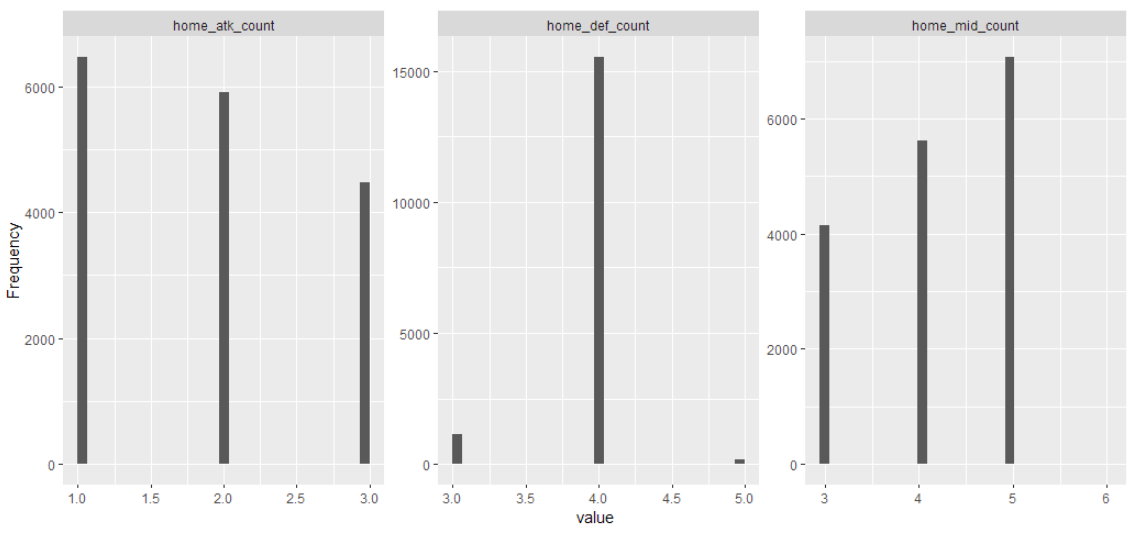
\includegraphics[scale=0.6]{images/04_01_roles_distribution.png}
	\caption[Distribuzione dei ruoli nelle partite]{Distribuzione dei ruoli nelle partite}
\end{figure}

\begin{figure}[H]
	\centering
	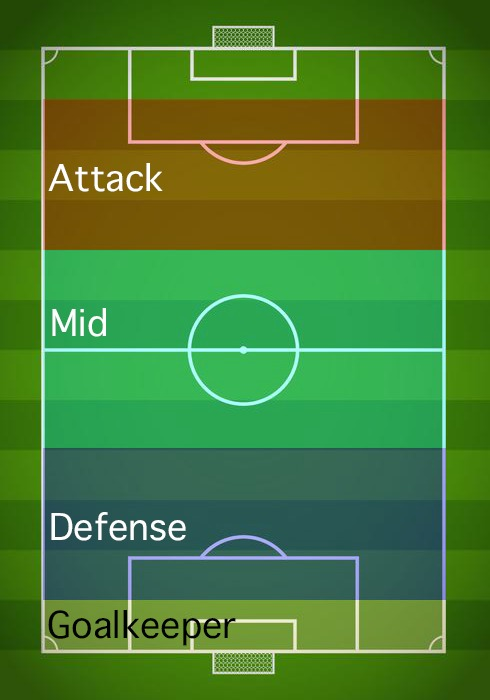
\includegraphics[scale=0.4]{images/soccer-field-horizontal.png}
	\caption[Suddivisione del campo da calcio in ruoli]{Suddivisione del campo da calcio in ruoli}
	\label{fig:soccer-field}
\end{figure}


\subsubsection{Potenzialità di una squadra in partita}

Se in \textit{PlayerAttributes} (le cui colonne sono meglio descritte nella tabella \ref{tab:player_attr}) vengono espresse quasi 40 diverse abilità tipiche dei giocatori di calcio, non tutte sono essenziali per ciascun ruolo. Si trovano ad esempio \texttt{finishing} e \texttt{shot\_power} come caratteristiche degli attaccanti oppure \texttt{marking} e \texttt{standing\_tackle} per i difensori, e ancora altri attributi espressamente dedicati ai portieri.

In questo contesto, si è pensato di computare per ciascuna partita e squadra partecipante diversi punteggi per esprimere la potenza di una certa squadra, sulla base dei 4 ruoli disponibili nel calcio: \textbf{portiere}, \textbf{difesa}, \textbf{centrocampo} e \textbf{attacco}. Tali punteggi costituiranno in seguito i nodi della Rete Bayesiana su cui fare le dovute predizioni; si è deciso di calcolarli sfruttando i valori registrati dai giocatori che costituiscono i 4 ruoli della squadra durante una partita.

\vspace{3ex}

Inizialmente, si era pensato di assegnare a ciascun giocatore della partita un determinato punteggio calcolato attraverso una media pesata delle abilità più rilevanti per il ruolo che si sta giocando. Questo avrebbe comportato la necessità di aggregare per ciascun giocatore diverse abilità a seconda del suo ruolo in partita, per successivamente andare a costituire un'ulteriore aggregazione di tutti i giocatori in una certa posizione al fine di computare le potenzialità della squadra, per ciascun ruolo, durante la partita. 

Seppur il calcolo sia logicamente sensato, conoscendo il dominio si è tuttavia ragionato sul fatto che ciascun giocatore del calcio moderno è sempre intrinsecamente legato ad un ruolo, che assume in tutte le partite da egli giocate. Seguendo questo ragionamento si è conseguentemente provato a verificare l'attendibilità del punteggio \texttt{overall\_rating}, già espresso all'interno del dataset per ciascun giocatore, che dovrebbe rappresentare il punteggio generale del giocatore con particolare attenzione al proprio ruolo. 

É stata pertanto condotta un'analisi di correlazione fra \texttt{overall\_rating} e gli altri attributi di \textit{PlayerAttribute} per dimostrare che il primo fosse in grado di adattarsi efficacemente al tipico ruolo del giocatore considerato. Tale analisi, presentata nella sezione successiva, ha chiaramente evidenziato che l'attributo \texttt{overall\_rating} della tabella \textit{PlayerAttribute} è sufficiente a descrivere efficaciemente un giocatore, pertanto si è scelto di utilizzare questa colonna come unica caratteristica per costituire i punteggi aggregati di difesa, centrocampo e attacco. 


\subsubsection{Correlazione fra ruolo e \texttt{overall\_rating}}

Per analizzare la correlazione fra ruolo di un giocatore e \texttt{overall\_rating}, al fine di comprendere se quest'ultimo sia adatto a descrivere efficamente un giocatore, si è innanzitutto tentato di suddividere i giocatori in ruoli, sulla base dei valori assunti in determinate abilità e studiando la distribuzione dei valori assunti da quest'ultime.

Facendo riferimento a \texttt{gk\_diving} e la figura \ref{img:dataset-gkdiving-distr}, si è facilmente evidenziata una distribuzione nettamente suddivisa fra valori sopra 50 (su una scala di 100) e sotto 40, a scindere inequivocabilmente i giocatori portieri da tutti gli altri. Per questi, è chiaramente evidente in figura \ref{img:dataset-gk-corr} che \texttt{overall\_rating} sia totalmente dipendente dalle abilità legate al portiere e dalla capacità di reagire rapidamente.

\begin{figure}[H]
	\centering
	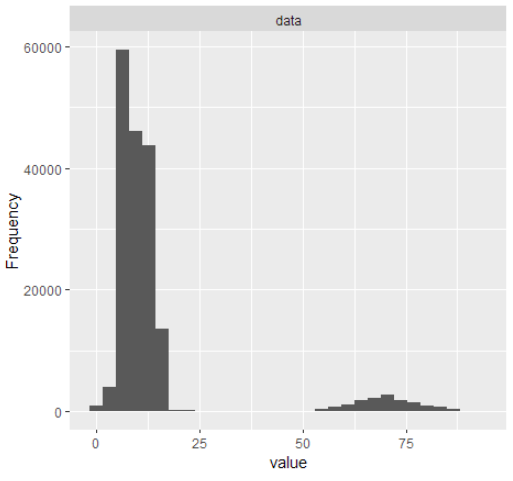
\includegraphics[scale=0.65]{images/04_02_gkdiving_distribution.png}
	\caption[Distribuzione di \texttt{gk\_diving}]{Distribuzione di \texttt{gk\_diving}}
	\label{img:dataset-gkdiving-distr}
\end{figure}

\begin{figure}[H]
	\centering
	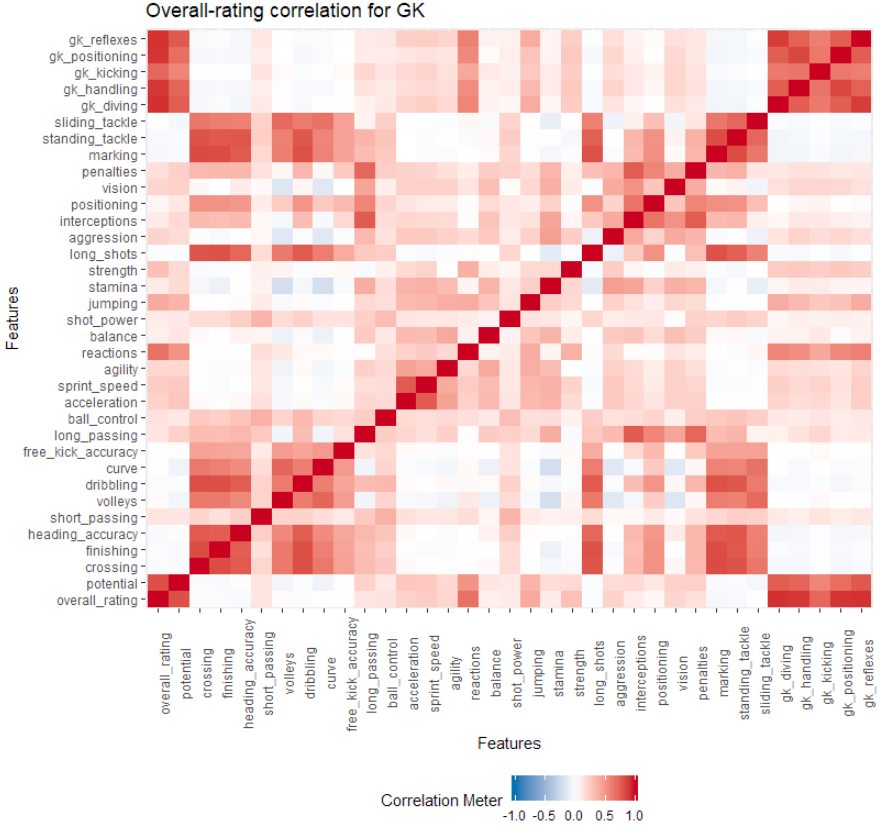
\includegraphics[scale=0.8]{images/04_03_gk_corr.png}
	\caption[Correlazione fra \texttt{overall\_rating} (prima riga dal basso) e le abilità di un portiere (a destra)]{Correlazione fra \texttt{overall\_rating} (prima riga dal basso) e le abilità di un portiere (a destra)}
	\label{img:dataset-gk-corr}
\end{figure}

Studiando invece la correlazione fra le diverse abilità, si è evinto che due fra gli attributi meno correlati fra loro fossero \texttt{marking} e \texttt{finishing}, associati rispettivamente al ruolo difensivo e quello d'attacco. Sfruttando l'incorrelazione di -0.62 qui mostrata, si è quindi potuto sfruttare i due campi per scindere il dataset dei giocatori in attaccanti e difensori, per studiarne il comportamento di \texttt{overall\_rating}.

\begin{verbatim}
cor(PlayerAttributes[PlayerAttributes$gk_diving <= 40, ]$marking,
PlayerAttributes[PlayerAttributes$gk_diving <= 40, ]$finishing,
use ="pairwise.complete.obs"); 		RESULT = -0.6204823
\end{verbatim}

In figura \ref{img:dataset-def-corr} è possibile osservare la matrice di correlazione applicata sui difensori, cioè i giocatori non-portieri con un punteggio minimo di 50 su \texttt{marking} e massimo di 50 su \texttt{finishing}. Si evince come la maggior parte della correlazione di \texttt{overall\_rating} (prima riga dal basso) la si ottenga con le abilità tipiche della difesa come \texttt{marking}, \texttt{sliding\_tackle} e \texttt{interceptions}. Le abilità del portiere sono totalmente ininfluenti ed in generale anche le caratteristiche d'attacco non sono molto rilevanti.

\begin{figure}[H]
	\centering
	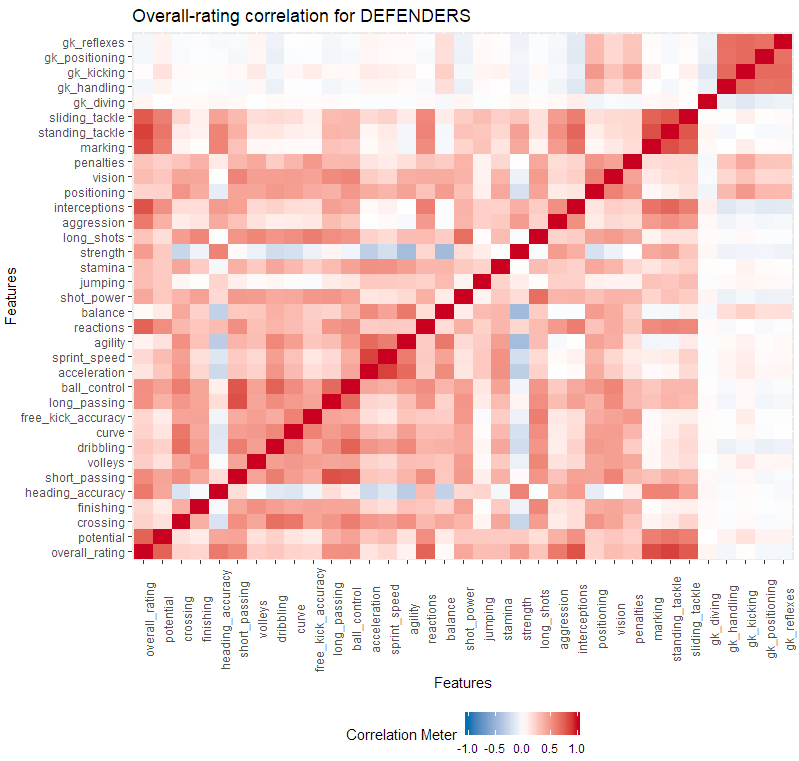
\includegraphics[scale=0.8]{images/04_04_def_corr.png}
	\caption[Correlazione fra \texttt{overall\_rating} (prima riga dal basso) e le abilità di un difensore]{Correlazione fra \texttt{overall\_rating} (prima riga dal basso) e le abilità di un difensore}
	\label{img:dataset-def-corr}
\end{figure}

Infine, nella figura \ref{img:dataset-atk-corr} viene presentata la correlazione fra \texttt{overall\_rating} e le abilità di un attaccante, cioè un giocatore non-portiere con un punteggio massimo di 50 su \texttt{marking} e minimo di 50 su \texttt{finishing}. Questa volta si nota che le abilità difensive non hanno alcuna influenza sul punteggio globale, a differenza di quanto avvenga invece per le abilità più legate ai tiri in porta, al dribbling e alla velocità di corsa, che erano decisamente meno influenti per i difensori.

\begin{figure}[H]
	\centering
	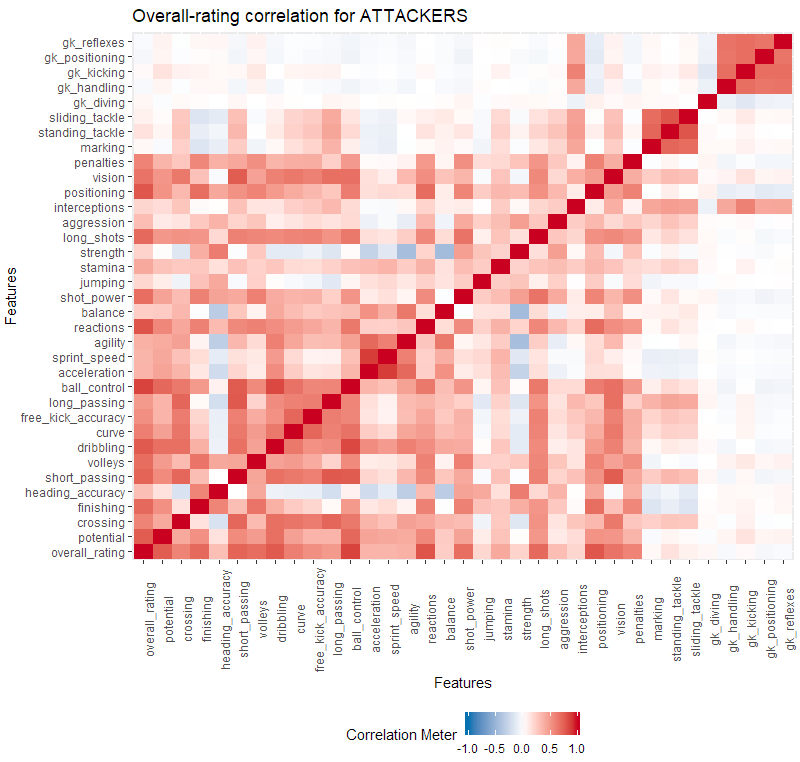
\includegraphics[scale=0.8]{images/04_05_atk_corr.png}
	\caption[Correlazione fra \texttt{overall\_rating} (prima riga dal basso) e le abilità di un attaccante]{Correlazione fra \texttt{overall\_rating} (prima riga dal basso) e le abilità di un attaccante}
	\label{img:dataset-atk-corr}
\end{figure}


\clearpage
\subsubsection{Calcolo e discretizzazione dei punteggi generali per la squadra}
\label{sec:dataset-discr}

Tramite le precedenti considerazioni si è dimostrato che è possibile utilizzare il solo attributo \texttt{overall\_rating} per descrivere efficacemente un giocatore. Per calcolare quindi i punteggi ottenuti da una certa squadra, composta dagli 11 giocatori, in una certa partita si è quindi pensato di mediare fra loro gli \texttt{overall\_rating} dei giocaori facenti parte dei 4 diversi ruoli del calcio.

Così facendo si sono ottenuti 4 valori continui, da 1 a 100, rappresentanti le caratteristiche generali della squadra sulla base dei giocatori coinvolti nella partita. Successivamente verrà dimostrato che, per il caso in esame, considerare anche il numero di giocatori in un determinato ruolo è ininfluente.

Al fine di sottoporre queste informazioni ad una Rete Bayesiana, si è quindi proceduto con una discretizzazione dei valori ottenuti, che erano compresi fra 1 e 100. Inizialmente, si è scelto di utilizzare 4 intervalli di discretizzazione; più avanti in questo elaborato (nella sezione \ref{sec:perf-discret}) si mostrerà come questa scelta possa avere un'influenza sulle performance del modello di predizione.

\vspace{5ex}

I dati ottenuti sono stati ripuliti delle informazioni non più rilevanti, come i dati sui singoli giocatori, e quindi esportati in formato CSV per essere sottoposti alla Rete Bayesiana con lo scopo di fare previsioni sul risultato di una partita e inferenze di diverso genere sui possibili valori assunti dai 4 punteggi per ciascuna squadra.



\clearpage



\section{Rete Bayesiana}

Lo scopo di questo progetto è la predizione del risultato di una partita di calcio. Sfruttando i dati ottenuti dal dataset d'origine attraverso l'elaborazione esplicata nel dettaglio alla sezione \ref{sec:dataset-elab}, è possibile costruire un modello di apprendimento che utilizzi le caratteristiche tecniche delle due squadre in competizione per predire, su base statistica, chi sarà il vincitore.

A questo scopo di è scelto di utilizzare una Rete Bayesiana, un modello grafico probabilistico che rappresenta un insieme di variabili stocastiche con le loro dipendenze condizionali attraverso l'uso di un grafo aciclico diretto (DAG). Nel caso in esame, le variabili stocastiche sono rappresentate proprio dai punteggi assunti dalla squadra in casa e quella in trasferta nei 4 ruoli tipici del calcio. 

In questo capitolo vi si farà riferimento con la seguente nomenclatura: \\
\texttt{HOME\_GK}, \texttt{HOME\_DEF}, \texttt{HOME\_MID} e \texttt{HOME\_ATK} per la squadra che gioca in casa e \\
\texttt{AWAY\_GK}, \texttt{AWAY\_DEF}, \texttt{AWAY\_MID} e \texttt{AWAY\_ATK} per la squadra ospite.
La variabile target, cioè quella da predire, verrà invece identificata come \texttt{WINNER}.



\subsection{Assunzioni}
\label{sec:bn-assumptions}

La principale assunzione su cui si basa l'intero lavoro di modellazione con le Reti Bayesiane è costituito dal fatto che le due squadre che si sfidano in una partita sono fra loro causalmente indipendenti. Ciò significa che le variabili stocastiche della squadra in casa, e quindi i nodi che compongono la Rete Bayesiana, non devono poter essere raggiungibili attraverso un cammino orientato da parte dei nodi costituenti la squadra in trasferta, e viceversa.

In altre parole, se ciascuna squadra è rappresentata da un arbitrario numero di nodi, questi costituiranno una sorta di componente connessa che interagirà con le altre solamente attraverso dei nodi intermedi con soli archi entranti. Il risultato della partita è un tipico nodo di collegamento fra le due squadre, i cui punteggi che le caratterizzano nei diversi ruoli non si influenzano fra una squadra l'altra.



\subsection{Software}

Il linguaggio di programmazione utilizzato per la modellazione della Rete Bayesiana su cui effettuare le predizioni è R\cite{site:r}, un ambiente software gratuito per computazione di natura statistica. Più nello specifico, la libreria utilizzata per lo scopo del progetto è \texttt{bnlearn}\cite{site:bnlearn}, pensata proprio per lavorare con modelli di apprendimento basati sulle Reti Bayesiane.

\texttt{bnlearn} mette a disposizione una moltitudine di istruzioni sia per strutturare la Rete che per svolgere predizioni e inferenze di qualsiasi tipo. Fra le funzionalità più vantaggiose, la libreria è in grado di generare anche la struttura fisica della rete basandosi sui dati conosciuti e vantando la capacità di sfruttare più che una decina di algoritmi di apprendimento della struttura. Inoltre, \texttt{bnlearn} è in grado di lavorare anche con dataset continui. 

La libreria è il principale punto di riferimento per l'utilizzo delle Reti Bayesiane in R ed è stata creata da Marco Scutari, italiano specialista del settore oggi occupato all'Istituto Dalle Molle di Studi sull'Intelligenza Artificiale di Lugano.

\vspace{3ex}

Altre librerie utilizzate durante lo sviluppo ed in particolare per la fase di pre-analisi ed elaborazione descritta nel precedente capitolo sono \texttt{DataExplorer}, \texttt{arules} e \texttt{caret} per la visualizzazione e lavorazione dei dati.



\subsection{Progettazione di una rete}

Come precedentemente accennato, con \texttt{bnlearn} è possibile modellare una Rete Bayesiana sia progettandola in autonomia che facendola generare automaticamente alla libreria con la possibilità di sfruttare una moltitudine di approcci diversi.

Gli step per la progrettazione di una Rete sono in primis la modellazione della sua struttura e poi la specifica dei parametri, ossia delle probabilità condizionate di ciascun nodo (CPT). Una peculiarità delle Reti Bayesiane, se confrontate ad altri modelli con cui è possibile fare Machine Learning, è quella di essere completamente visibile agli occhi del programmatore e soprattutto semanticamente significativa, specie per quanto riguarda il DAG rappresentante la struttura della rete stessa. \'E importante che il grafo della Rete non sia particolarmente complesso, sia per facilitarne la lettura che per evitare un peggioramento delle performance incontrollato.



\subsection{Generazione della struttura}

Nel caso in esame, si è deciso di sfruttare in primis una rete auto generata dai dati a disposizione. Ciò ha il vantaggio di essere immediatamente funzionante e tendenzialmente cablata per avere delle prestazioni quasi ottimali. La generazione delle struttura avviene tramite un approccio data-driven, sfruttando il dataset su cui si vuole fare predizioni e inferenze. All'approccio numerico basato sui dati, segue spesso un \textit{tuning} effettuato sulla conoscenza del dominio di riferimento, come possono essere ad esempio determinate assunzioni fatte a priori.


\subsubsection{Algoritmo di apprendimento}

\texttt{bnlearn} mette a disposizione del programmatore svariati metodi per l'apprendimento della struttura della Rete: \textit{constraint-based}, \textit{score-based} e \textit{hybrid}. Partendo da una condizione iniziale di indecisione relativo al metodo migliore da utilizzare per il progetto in esame, si è scelto di utilizzare un approccio empirico basato sulla sperimentazione. Provando svariati algoritmi, si è notato che molti di questi lasciavano all'interno della rete dei nodi completamente isolati, motivo per cui sono stati scartati a priori.

Fra i metodi che sono sembrati più "corretti" nella generazione della Rete è emerso \textit{hill-climbing} (HC), un algoritmo \textit{score-based} di ricerca greedy che parte da una condizione di rete senza archi, a cui vengono progressivamente aggiunti, rimossi o invertiti fino alla generazione di una rete che non riesce a ottenere un punteggio migliore. Quest'ultimo è calcolato attraverso una funzione di ottimizzazione applicata alla rete stessa ed utilizzata per apprendere la struttura sub-ottimale\cite{thesis:bnlearn-marco}.

\begin{figure}[H]
	\centering
	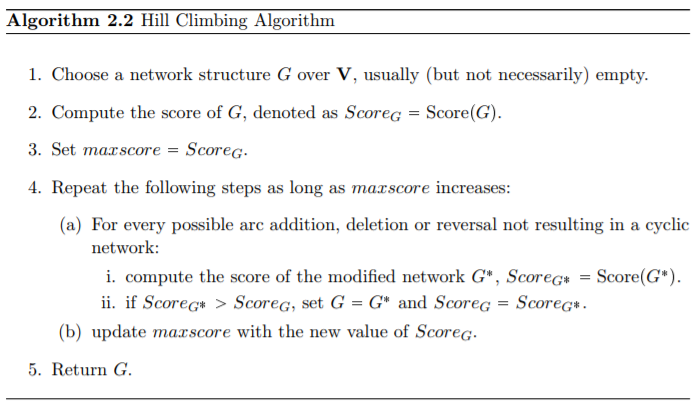
\includegraphics[scale=1]{images/05_00_hc_algo.png}
	\caption[Algoritmo Hill Climbing per l'apprendimento della struttura di una BN]{Algoritmo Hill Climbing per l'apprendimento della struttura di una BN}
	\label{img:hc-algorithm}
\end{figure}


\clearpage
\subsubsection{Autogenerazione}

Il codice per la generazione e visualizzazione della struttura della Rete Bayesiana con \texttt{bnlearn} è decisamente semplice, e porta al risultato mostrato nella figura \ref{img:hc-pure}:

\begin{verbatim}
dag = hc(dataset);
plot(dag);
\end{verbatim}

\begin{figure}[H]
	\centering
	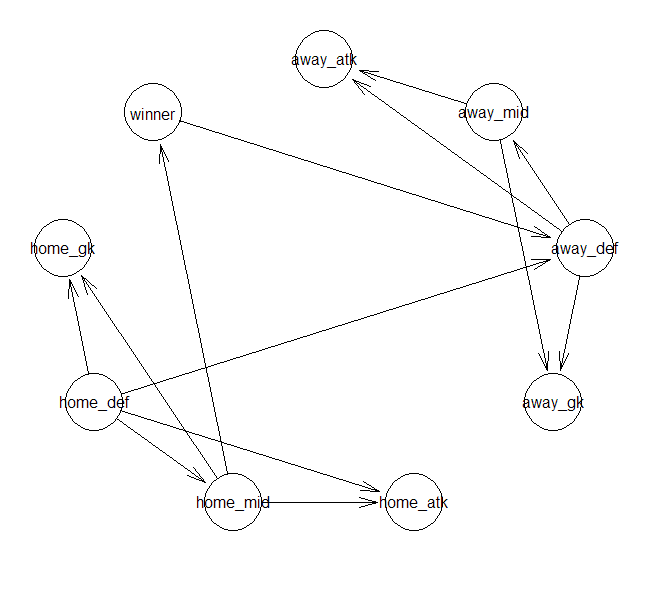
\includegraphics[scale=0.75]{images/05_01_hc_pure.png}
	\caption[Rete autogenerata con algoritmo HC]{Rete autogenerata con algoritmo HC}
	\label{img:hc-pure}
\end{figure}

Nonostante la rete generata (figura \ref{img:hc-pure}) appaia semplice e piuttosto sensata, è doveroso far notare che alcuni archi contraddicono le assunzioni fatte nella sezione \ref{sec:bn-assumptions} per cui è stato detto che le due squadre in competizione devono essere composte da nodi causalmente indipendenti. Come si vede nell'immagine, \texttt{HOME\_MID} ha un arco entrante in \texttt{AWAY\_DEF} e come se non bastasse anche \texttt{WINNER}, la variabile target, va a finire dentro il medesimo nodo. Per questo motivo, si è dimostrato necessario introdurre un intervento manuale per la generazione della rete.


\clearpage
\subsubsection{Vincoli di generazione}

Attraverso \texttt{bnlearn} è possibile specificare alcuni vincoli riguardanti la creazione automatica della struttura della Rete, sia in termini di archi da evitare che di archi da includere nella struttura stessa.

Sfruttando un parametro chiamato \texttt{blacklist}, è stata fornita alla funzione \texttt{hc} una lista di archi da \textbf{non} includere nella rete. Così facendo è stato possibile impedire alle due squadre di collegarsi fra loro, come scelto nelle assunzioni. \\
Di seguito viene mostrato il codice che genera la rete in figura \ref{img:hc-bl}.

\begin{verbatim}
home_attr = c("home_gk", "home_def", "home_mid", "home_atk");
away_attr = c("away_gk", "away_def", "away_mid", "away_atk");
bl = rbind(
           as.matrix(expand.grid(home_attr, away_attr)),
           as.matrix(expand.grid(away_attr, home_attr))
dag = hc(dfull1, blacklist = bl);
\end{verbatim}

\begin{figure}[H]
	\centering
	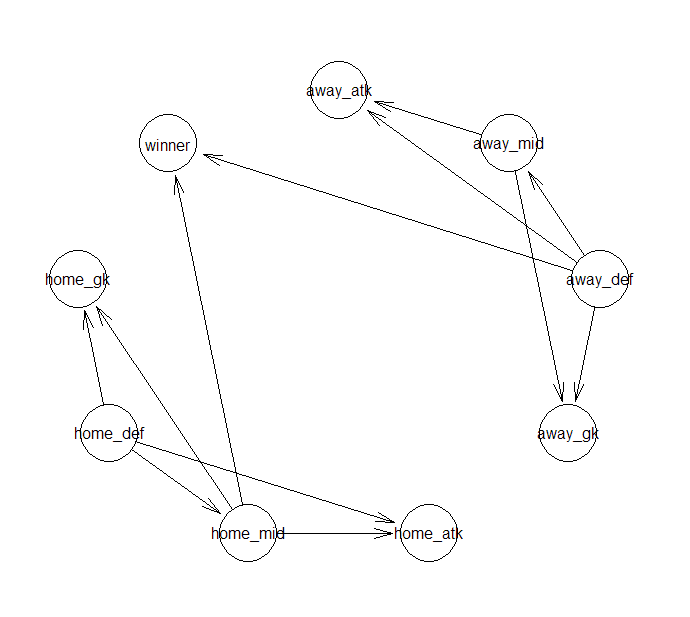
\includegraphics[scale=0.8]{images/05_02_hc_bl.png}
	\caption[Rete autogenerata con algoritmo HC e blacklist per evitare che le due squadre si connettessero fra loro]{Rete autogenerata con algoritmo HC e blacklist per evitare che le due squadre si connettessero fra loro}
	\label{img:hc-bl}
\end{figure}

Questa volta, le due squadre sono causalmente indipendenti e quindi le assunzioni sono rispettate. Inoltre, è possibile notare che solamente uno dei nodi di entrambe le squadre va a costituire una dipendenza causale diretta con la variabile target, cioè \texttt{HOME\_MID} e \texttt{AWAY\_DEF}. Non vi è una vera e propria spiegazione semantica a questo fenomeno, ma intuitivamente si potrebbe pensare che mentre una squadra, quella in casa, punti con questa rete a massimizzare le proprie capacità di possesso palla e attacco (con il centrocampo), l'altra sia prevalentemente interessata a difendersi.

Questo tipo di comportamento è sicuramente originato dal dataset a disposizione, probabilmente anche a causa del fatto che la distribuzione della variabile \texttt{WINNER} è mal condizionata: circa nel 50\% dei casi vince la squadra in casa, mentre solamente il 25\% delle partite è vinta da quella in trasferta, con la rimanente porzione di pareggi.

Quest'ultima intuizione potrebbe essere confermata dal fatto che, riducento il problema ternario \texttt{WINNER}=\textit{home/away/draw} ad un problema binario \texttt{WINNER}=\textit{home/not home}, la rete cambia nuovamente e questa volta sono entrambi i centrocampi ad influenzare direttamente il target. Lo si può vedere in figura \ref{img:hc-bin-bl}.

\begin{figure}[H]
	\centering
	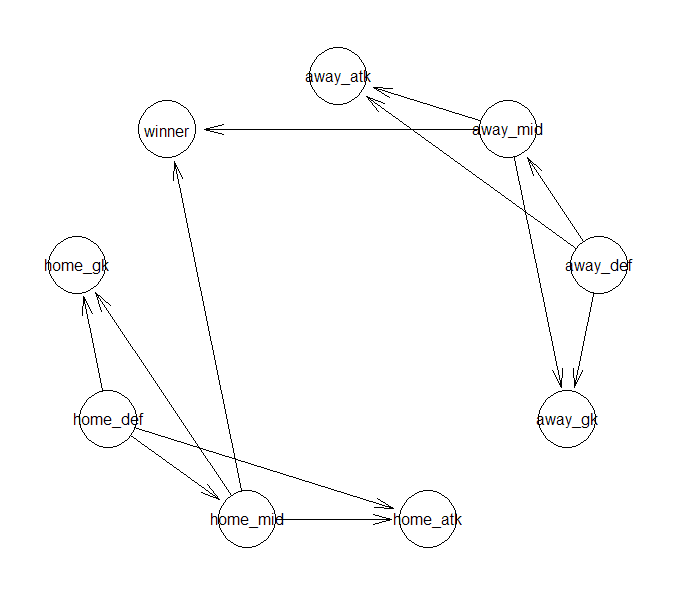
\includegraphics[scale=0.75]{images/05_02_hc_bin_bl.png}
	\caption[Rete autogenerata con algoritmo HC e blacklist sul problema binario]{Rete autogenerata con algoritmo HC e blacklist sul problema binario}
	\label{img:hc-bin-bl}
\end{figure}

Si vedranno più avanti in questo elaborato le implicazioni sulle performance derivate dalla considerazione di un problema binario piuttosto che ternario, o viceversa.


\subsection{Generazione delle CPT}

Appresa (o manualmente generata) la struttura della Rete, è quindi necessario fissare i parametri, cioè le probabilità condizionate di ciascun nodo. Grazie alla proprietà di Markov per cui un nodo è influenzato solo localmente dai nodi facenti parte del suo Markov Blanket, calcolare le CPT è un'operazione relativamente rapida se, come in questo caso, i nodi non hanno un numero particolarmente elevato di archi entranti. Questa proprietà rappresenta un considerevole vantaggio, perché significa che la complessità di calcolare i parametri della rete non cresce con la dimensione della rete ma solamente con il numero di nodi localmente dipendenti.

Anche in questo caso, \texttt{bnlearn} fornisce un'istruzione decisamente comoda per la stima dei parametri basandosi sui dati, qui mostrata:

\begin{verbatim}
fitted = bn.fit(dag, dtrain);
\end{verbatim}

A differenza di quanto avviene per la generazione della struttura, l'apprendimento dei parametri dovrebbe essere eseguito solamente sul training set.


\subsection{Predizione e inferenza}

Una volta generate sia la struttura che i parametri della Rete Bayesiana è finalmente possibile effettuare predizioni e inferenze con il modello appreso. Ancora una volta, le istruzioni sono di semplice utilizzo. 

\vspace{3ex}

La funzione \texttt{predict(object, node, data, method)} permette di generare un insieme di predizioni per una data variabile e successivamente verificare quanto predetto sia coerente con il test set.

\begin{verbatim}
pred = predict(fitted, "winner", dtest);
cat("Accuracy:", mean(pred == dtest$winner, na.rm = TRUE));
\end{verbatim}

\vspace{3ex}

La funzione \texttt{cpquery(fitted, event, evidence, cluster, method)} consente invece di effettuare inferenze, calcolando la probabilità che un evento si verifichi date le evidenze, sfruttando il modello appreso.

\begin{verbatim}
res = cpquery(
      fitted,
      event = (winner == "home"),
      evidence = ((home_mid == "terrible") & (away_def == "good")));
print(res);
\end{verbatim}

\vspace{2ex}

Per completezza, si cita qui anche la funzione \texttt{cpdist}, con firma identica a quella di \texttt{cpquery}, ma volta alla generazione di campioni casuali date le evidenze e in accordo con le CPT dei nodi di volta in volta campionati.


\subsubsection{Qualche esempio}

A scopo dimostrativo, si presentano in questa sede alcune delle inferenze che è possibile produrre attraverso la libreria \texttt{bnlearn} e l'ultima rete mostrata. I seguenti esempi sono stati generati attraverso l'interfaccia grafica che sarà spiegata nel capitolo \ref{sec:ui}.

\begin{verbatim}
P(winner = home | home_mid = terrible, away_mid = good) = 0.184466
P(winner = home | home_mid = terrible, away_mid = terrible) = 0.3825503
P(winner = home | home_mid = terrible, away_mid = excellent) = 0.1244541
P(winner = home | home_gk = very good, away_gk = terrible) = 0.6796657
P(winner = home | home_atk = good, away_gk = excellent) = 0.3128295
P(winner = home | home_atk = good, away_gk = good) = 0.4764493
P(winner = not home | home_mid = terrible, away_mid = excellent) = 0.908642
\end{verbatim}

Dai risultati, è possibile facilmente notare come la Rete sia in grado di stimare la probabilità che la squadra di casa sia vincente, sulla base dei valori attribuiti alle diverse variabili secondo la discretizzazione che sarà spiegata nel capitolo \ref{sec:perf-discret}. Gli esempi considerano il problema binario, per cui la squadra che gioca in casa può vincere o non vincere (ma senza sapere se si tratti di un pareggio o una sconfitta).



\clearpage



\section{Performance}

Quando si modellano delle Reti Bayesiane e si sceglie di auto-generare la struttura della rete o comunque provare diverse possibili strutture, è essenziale sfruttare un approccio di tipo sperimentale per determinare, al netto delle assunzioni, quale possa rappresentare la soluzione migliore dal punto di vista delle prestazioni ottenute.

Queste prevedono la necessità di tenere in considerazione diverse metriche standard, che esprimono la bontà di un modello di apprendimento e quindi di predizione sui risultati futuri. Ciò è possibile suddividendo in due (o più) parti il dataset che si vuole fornire all'algoritmo di stima dei parametri della Rete. Ricavando un training set su cui addestrare il modello predittivo e successivamente un test set tramite il quale provare il modello generato, è possibile quindi dedurre le metriche di valutazione.

Al fine di valutare diversi modelli da adottare per questo progetto, le analisi preliminari sulle varie possibilità sono state effettuate attraverso una suddivisione del dataset in 75\% per il tranining set e 25\% per il test set; successivamente, una k-fold cross validation è stata utilizzata per ottenere valutazioni più accurate.



\subsection{Ricerca della soluzione migliore}

La ricerca del modello di apprendimento migliore, sia in termini di elaborazione dei dati che generazione della Rete Bayesiana, ha seguito un'evoluzione graduale volta ad individuare la soluzione più accurata per le predizioni sul test set. Questo tipo di valutazione ha coinvolto diversi aspetti che sono di seguito presentati.


\subsubsection{Tempi}

Un importante aspetto da considerare quando si ha a che fare con modelli di apprendimento, e più in generale con qualsiasi tipo di Machine Learning, è il tempo necessario per imparare i parametri del modello e successivamente stimare il target di nuove istanze. In questo caso specifico, sia l'algoritmo per la generazione della Rete che per la stima dei parametri si sono rivelati decisamente performanti.

L'apprendimento della struttura della Rete è quasi istantaneo per tutti gli algoritmi provati, con tempi di esecuzione prossimi allo zero. L'apprendimento dei parametri della Rete, e quindi delle CPT, richiede invece tempi differenti a seconda della complessità della struttura. I grafi presentati nel capitolo precedente hanno richiesto sempre meno di un secondo per la stima delle CPT. Tale complessità aumenta non con la dimensione della Rete ma con l'aumentare della dipendenza causale (locale) delle variabili stocastiche, quindi nel momento in cui si tenta di stimare i parametri di una Rete nella quale i nodi che ne fanno parte hanno un considerevole numero di genitori; verrà presentato in seguito un esempio di questo tipo di Rete.

Anche i tempi per effettuare predizioni e inferenze sul modello già appreso sono pressoché insignificanti per tutte le alternative provate.

Alla luce di queste considerazioni, il tempo è una metrica piuttosto ininfluente per il caso in esame. L'unica accortezza necessaria è quella di evitare la generazione di strutture particolarmente dense di connessioni, pratica che rappresenta comunque una cattiva scelta anche dal punto di vista dell'accuratezza del modello che ne risulterebbe.


\subsubsection{Problema ternario o binario}

Come accennato nel precedente capitolo, il dataset utilizzato per apprendere la struttura e i parametri della Rete Bayesiana presenta una cattiva distribuzione per la variabile target \texttt{WINNER}. Come mostrato in figura \ref{img:perf-target-distr}, la maggior parte delle partite considerate sono state vinte da parte della squadra in casa, mentre la rimanente parte è quasi equamente suddivisa fra pareggi e vittoria per la squadra in trasferta.

\begin{figure}[H]
	\centering
	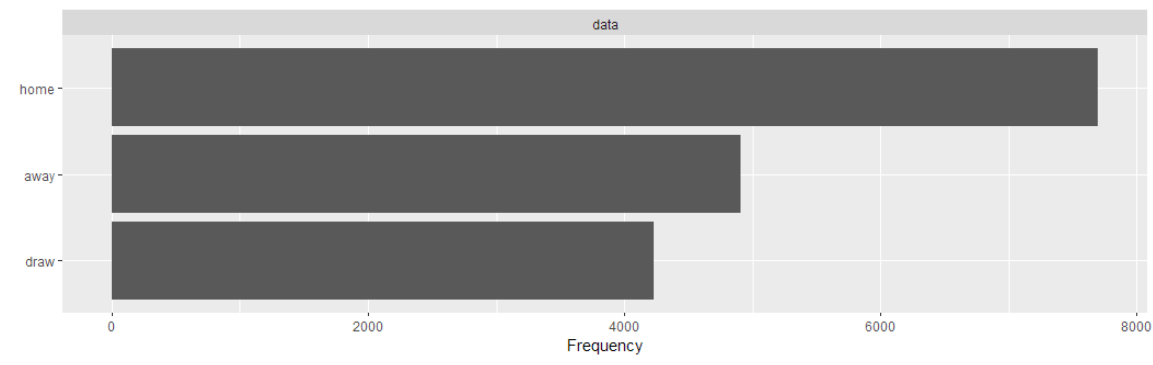
\includegraphics[scale=0.6]{images/06_01_target-distr.png}
	\caption[Distribuzione della variabile target]{Distribuzione della variabile target}
	\label{img:perf-target-distr}
\end{figure}

Considerata tale distribuzione e il dominio del problema, è facile aspettarsi che per un modello di predizione possa essere complesso determinare quali siano i casi nei quali a vincere è la squadra ospite o, ancor peggio, si ottenga un pareggio. Il calcio infatti non è chiaramente una scienza esatta, motivo per cui le statistiche delle due squadre non bastano autonomamente per determinare l'esito della partita, specialmente qualora queste abbiano caratteristiche simili; in egual modo, è difficile determinare le motivazioni per cui due squadre sulla carta molto diverse abbiano potuto terminare la partita con un egual numero di goal.

Per questi motivi, ci si aspetta che il modello di Rete Bayesiana abbia delle cattive performance proprio per quanto riguarda la predizione di un modello a tre classi (\texttt{WINNER} = \textit{home/away/draw}), ed in particolare con quanto ottenuto nelle due classi in minoranza. A dimostrazione di ciò, vengono presentate in tabella \ref{tab:10-fold-tern} le metriche di \textit{precision}, \textit{recall} e \textit{F1} calcolate come media di una 10-fold cross validation sulla Rete Bayesiana che era stata presentata in figura \ref{img:hc-bin-bl}.

\begin{table}[H]
	\centering
	\caption{10 fold cross validation sul problema ternario}
	\begin{tabular}{l|llll}
		\hline
		Classe & Precision & Recall & F1 \\
		\hline
		HOME & 0.5238946 & 0.849281 & 0.6477723 \\
		AWAY & 0.482222 & 0.4263695 & 0.4516147 \\
		DRAW & 0 & 0 & 0 \\
		\hline
	\end{tabular}
	\label{tab:10-fold-tern}
\end{table}

Nonostante l'\textit{accuracy} del modello sia del 0.5126, che non è un risultato particolarmente cattivo per un problema ternario di questo tipo, è possibile notare in tabella come i dati per la classe \textit{draw} siano pari a zero, indice del fatto che il modello non è mai in grado di predire una partita con risultato di pareggio.

\vspace{4ex}

Alla luce di questa considerazione, si è deciso di considerare per le prossime valutazioni solamente il problema di natura binaria in grado di predire se il vincitore di una partita sia la squadra in casa o meno; in quest'ultimo caso, non sarà dato sapere se il match sia più incline a concludersi con un pareggio o con la vittoria della squadra ospite. Come si vedrà nella sezione \ref{sec:perf-cross-fold} dedicata alla cross fold validation, il modello addestrato sul problema binario sarà in proporzione meno accurato, ma privo di mal condizionamenti causati da una cattiva distribuzione della variabile target nel dataset.


\subsubsection{Struttura della rete}

Per quanto riguarda la struttura della rete, si è scelto di considerare quella in figura \ref{img:hc-bin-bl} come punto di partenza, generata attraverso l'algoritmo \textit{hill climbing} sul problema binario, assicurandosi che le due squadre non avessero collegamenti diretti.

Poiché con tale configurazione le uniche variabili collegate al nodo target \texttt{WINNER} sono risultate \texttt{HOME\_MID} e \texttt{AWAY\_MID}, si è pensato di costituire una rete con un numero maggiore di collegamenti al nodo su cui effettuare le predizioni. Aumentando il numero di archi della Rete, aumenta conseguentemente anche il tempo necessario per la stima dei parametri.

Fra le varie alternative, nessuna è risultata in termini di \textit{accuracy} più performante rispetto alla Rete originale, che si attesta intorno al 60\%. Per questo motivo, si è dedotto che la rete ottenuta attraverso \textit{hill climbing} con un ridotto numero di archi fosse la migliore, e pertanto anche la semplicità della Rete stessa sia da preferire quando si ha a che fare con modelli Bayesiani.

Nella figura \ref{fig:hc-bin-all} è possibile osservare un esempio di Rete fra quelle testate, in cui tutti i nodi sono collegati alla variabile target secondo un'assunzione per cui ognuno di questi dovrebbe avere influenza sul risultato di una partita. Questa Rete si è rivelata tuttavia considerevolmente peggiore, con un'\textit{accuracy} intorno al 55\% e dei tempi di stima delle CPT decisamente più importanti, con alcune righe addirittura impossibili da calcolare.

\begin{figure}[H]
	\centering
	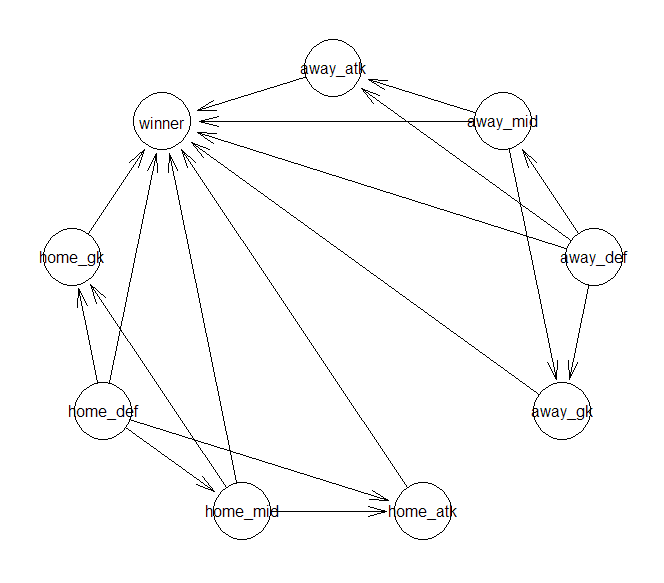
\includegraphics[scale=0.8]{images/06_02_hc_bin_wl_all.png}
	\caption[Rete che collega tutte le variabili al target]{Rete che collega tutte le variabili al target}
	\label{fig:hc-bin-all}
\end{figure}

\vspace{3ex}

Un ulteriore tentativo lo si è fatto tentando di aggiungere due nuove feature per ciascuna squadra, che raggruppassero rispettivamente il potenziale difensivo (portiere + difesa + mid) e offensivo (mid + attacco) delle squadre. Avendo provato a generare una Rete Bayesiana con questi nuovi nodi, si sono comunque ottenute performance totalmente simili alle precedenti, motivo per cui si è poi deciso di tornare alla configurazione della Rete originale.


\subsubsection{Discretizzazione delle features}
\label{sec:perf-discret}

Nonostante l'argomento di discretizzazione sia già stato affrontato nel capitolo \ref{sec:dataset-discr}, poiché si tratta di un'operazione da eseguire sui dati prima di fornirli alla Rete, tale argomento è tornato in auge per fare le ultime considerazioni sulle performance del modello. Infatti, il modo in cui vengono discretizzati i dati assume un ruolo fondamentale per l'intero processo di predizione, in quanto il modello sia in fase di apprendimento che di predizione sfrutta i valori assunti dalle variabili considerate ed espressi secondo la discretizzazione scelta.

Ci sono diversi metodi per discretizzare e per operare questo tipo di elaborazione si è utilizzato il package \texttt{arules} di R, che fra le più rilevanti mette a disposizione la discretizzazione \textit{fixed} e quella \textit{frequency-based}. Mentre la prima consente di specificare dei valori che costituiscono gli estremi degli intervalli di discretizzazione, il secondo metodo permette di effettuare una separazione automatica basata sulla distribuzione dei valori assunti dalla variabile che si sta discretizzando. L'obiettivo è quello di creare intervalli che contengano un numero bilanciato di campioni del dataset.

Considerata la distribuzione delle feature scelte per costruire la Rete Bayesiana, visibile nell'immagine \ref{fig:perf-scores-distr}, si è inizialmente pensato di discretizzare i valori in 4 intervalli. Particolare importanza è stata data alla scelta di un numero di intervalli pari, per evitare che troppe feature finissero nel valore centrale.

\begin{figure}[H]
	\centering
	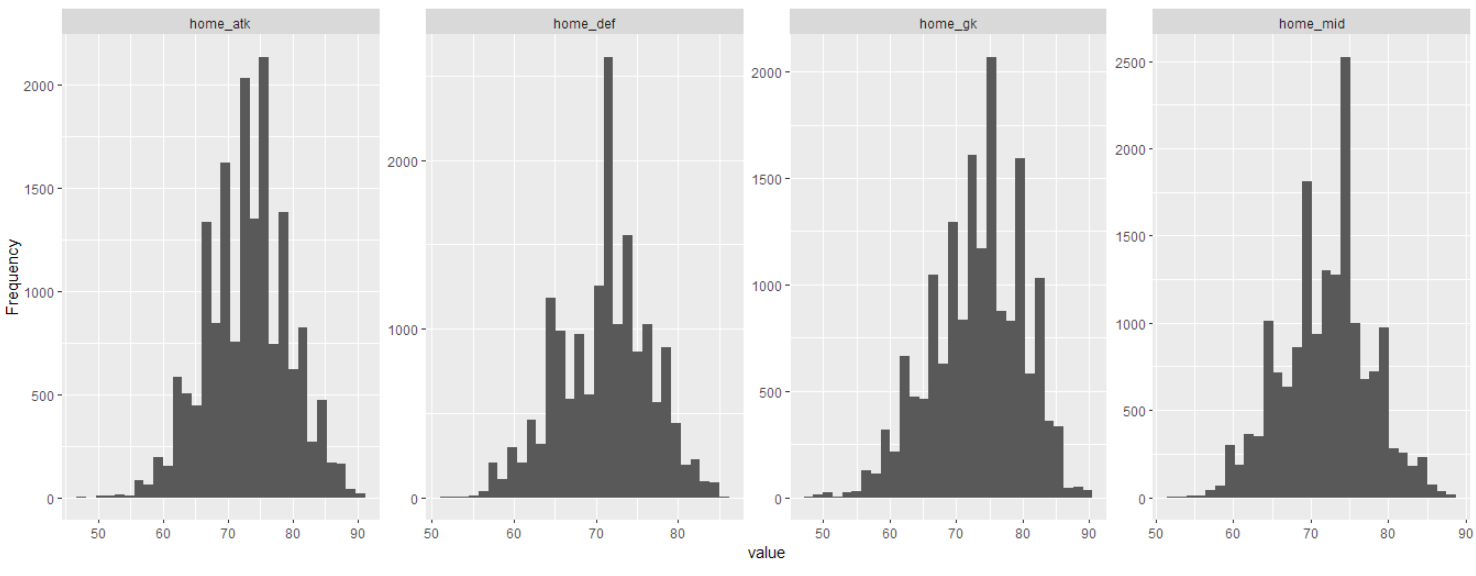
\includegraphics[scale=0.47]{images/06_03_score_distr.png}
	\caption[Distribuzione dei valori assunti dalle features]{Distribuzione dei valori assunti dalle features}
	\label{fig:perf-scores-distr}
\end{figure}

In seguito, poiché si è notato che i valori centrali delle feature fossero assunti da un gran numero di partite si è deciso di aumentare il numero di intervalli con cui discretizzare. Ciò ha portato ad un incremento nell'accuratezza dei modelli di predizione testati, motivo per cui si è rivelata un'intuizione vincente. Si è quindi scelto di delegare al pacchetto \texttt{arules} la scelta degli intervalli in maniera automatica attraverso un algoritmo basato sulla frequenza di distribuzione.

Si mostrano di seguito i limiti degli intervalli adottati per ciascun attributo della Rete e in figura \ref{fig:perf-discr-distr} anche la distribuzione assunta delle feature della squadra di casa in seguito alla discretizzazione. Si nota facilmente come il dataset si distribuisca equamente sui 6 intervalli creati, rinominati con delle etichette testuali e semanticamente rilevanti per agevolarne la lettura.

\begin{verbatim}
Discretization intervals for  home_gk :     48, 66, 71, 74, 77, 80, 90
Discretization intervals for  home_def :    52, 65, 69, 72, 74, 76, 86
Discretization intervals for  home_mid :    52, 66, 70, 72, 74, 77, 88
Discretization intervals for  home_atk :    48, 67, 70, 73, 76, 79, 91
Discretization intervals for  away_gk :     49, 66, 71, 74, 77, 80, 90
Discretization intervals for  away_def :    52, 65, 69, 72, 74, 76, 86
Discretization intervals for  away_mid :    51, 66, 70, 72, 74, 77, 89
Discretization intervals for  away_atk :    46, 67, 70, 73, 76, 79, 92
\end{verbatim}

\begin{figure}[H]
	\centering
	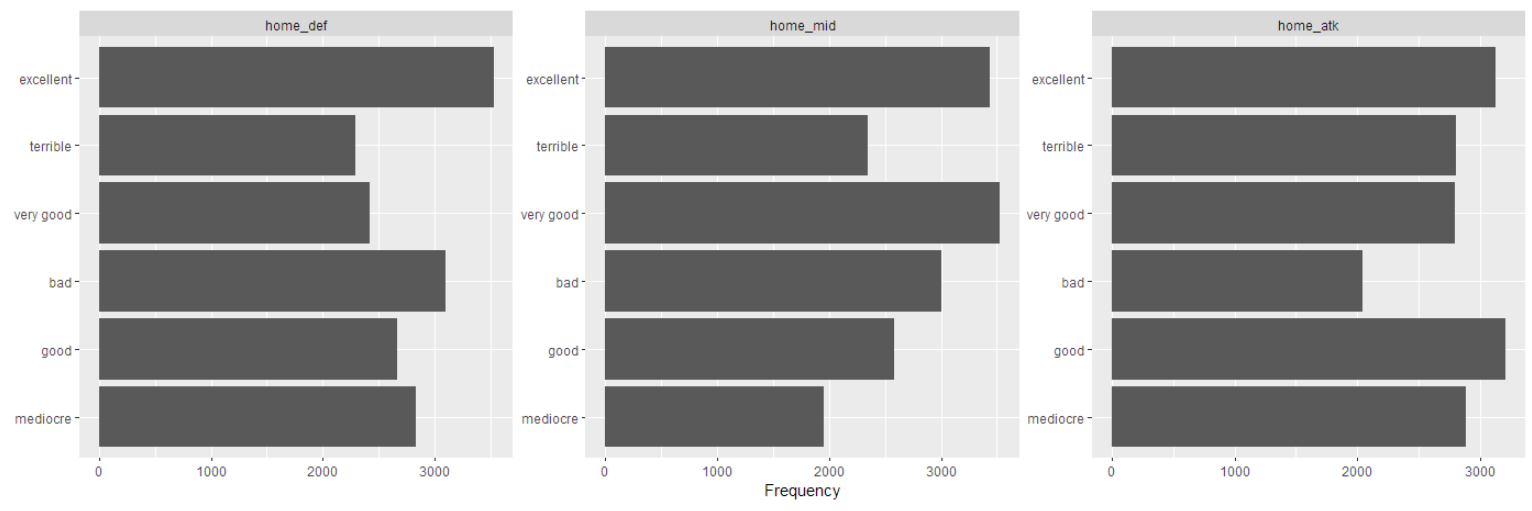
\includegraphics[scale=0.45]{images/06_04_discr_distr.png}
	\caption[Distribuzione dei valori assunti dalle features dopo la discretizzazione]{Distribuzione dei valori assunti dalle features dopo la discretizzazione}
	\label{fig:perf-discr-distr}
\end{figure}


\subsubsection{Differenti calcoli per il punteggio delle squadre}

Come ultimo tentativo di \textit{tuning} delle performance della rete si è provato a modificare il calcolo del punteggio assegnato a ciascuna squadra nei diversi ruoli calcistici. Si è rivalutato quanto spiegato nel capitolo \ref{sec:dataset-discr}, poiché ci si è resi conto che quel calcolo non tenesse conto del numero di giocatori in un certo ruolo ma solamente della media fra gli \texttt{overall\_rating}.

Al fine di pesare diversamente il punteggio ottenuto da una squadra per un determinato ruolo, ad esempio l'attacco, schierando 1 piuttosto che 4 giocatori in tal ruolo, si è deciso di applicare al calcolo della media una modifica che tenesse conto del numero di giocatori. Per pesare diversamente il beneficio ottenuto dall'aggiunta o la rimozione di giocatori in differenti ruoli, si è pensato di applicare un \textit{reward} logaritmico per ciascun giocatore, considerando la distribuzione media dei giocatori per ruolo (figura \ref{fig:dataset-roles-distr}) come situazione ottimale per costruire la formazione.

% TODO: calcolo overall_rating influenzato dal numero di giocatori per ruolo



\subsection{Cross Fold Validation}
\label{sec:perf-cross-fold}

Scelta la migliore elaborazione sulle feature da considerare e generata la struttura ottimale della Rete Bayesiana, abbiamo quindi applicato tutte le metriche di valutazione al modello appreso da \texttt{bnlearn}. In particolare, abbiamo deciso di implementare una cross fold validation sia attraverso una funzione di libreria, sia in maniera personalizzata.


\subsubsection{Funzione \texttt{bn.cv()}}

La libreria \texttt{bnlearn} mette a disposizione una comoda funzione \texttt{bn.cv(data, bn, loss)} per effettuare la cross fold validation. Questa consente di applicare diverse strategie di validazione e calcolare la \textit{loss} con svariati criteri di valutazione.

Per il progetto in esame, avendo a che fare con variabili di natura discreta si è optato per una \textit{loss} espressa come \textit{Classification Error} calcolata su una 10-fold validation standard. Tale \textit{loss} rappresenta l'errore di predizione per un singolo nodo, risultando quindi particolarmente indicata per valutare le performance della Rete nel predire la variabile target \texttt{WINNER}. Per il calcolo, viene sfruttata la proprietà di dipendenza locale della rete, quindi solo i genitori del nodo su cui si sta effettuando la predizione.

In seguito è riportato il codice per effettuare la cross validation e l'output della stessa, che riporta sia la struttura della rete che il valore di \textit{loss} ottenuto. Quest'ultimo è coerente con l'\textit{accuracy} che verrà mostrata nella sezione successiva.

\begin{verbatim}

cv = bn.cv(method = "k-fold", k = 10, data = dtest, bn = dag,
           loss = "pred", loss.args = list(target = "winner"));
print(cv)


k-fold cross-validation for Bayesian networks

target network structure:
[home_def][away_def][home_mid|home_def][away_mid|away_def]
[winner|home_mid:away_mid][home_gk|home_def:home_mid]
[home_atk|home_def:home_mid][away_gk|away_def:away_mid]
[away_atk|away_def:away_mid]

number of folds:                  10 
loss function:                    Classification Error 
training node:                    winner 
expected loss:                    0.3809976 
\end{verbatim}


\subsubsection{Accuracy, Precision e Recall}

Poiché la funzione integrata in \texttt{bnlearn} per la cross validation prevede come output solamente il valore della \textit{loss}, si è scelto di implementare anche una cross validation personalizzata per calcolare i valori di \textit{accuracy}, \textit{precision}, \textit{recall} e \textit{F1} al fine di valutare la bontà delle predizioni.

Calcolando tali valori su 10 fold e mediandone i risultati, si ottiene un'\textit{accuracy} del 62.57\% e le metriche riportate in tabella \ref{tab:10-fold-bin}. Queste tengono in considerazione la predizione della variabile \texttt{WINNER} con il valore \textit{home}, cioè considerando la squadra che gioca in casa come vincitrice.

\begin{table}[H]
	\centering
	\caption{10 fold cross validation SVM}
	\begin{tabular}{l|llll}
		\hline
		Classe & Precision & Recall & F1 \\
		\hline
		HOME & 0.636251 & 0.4293271 & 0.5117034  \\
		\hline
	\end{tabular}
	\label{tab:10-fold-bin}
\end{table}

A differenza di quanto mostrato in tabella \ref{tab:10-fold-tern} per il problema multiclasse, si può questa volta notare un peggioramento delle performance generali \textit{F1} per la classe \textit{home}, a fronte però di un risultato non completamente sbilanciato in sfavore di una certa classe, come accadeva per \textit{away} e \textit{draw} sul problema a tre classi.

Dalle metriche misurate si evince un valore accettabile di veri positivi nel considerare la squadra di casa vincente, ma anche una considerevole percentuale di falsi negativi.

Probabilmente ciò è dovuto all'effettiva difficoltà nel riuscire a predire il vincitore di una partita di calcio se ci si limita a osservare le caratteristiche dei giocatori che le compongono. Ciò accade perché molte volte si assiste a partite nelle quali le due squadre sfidanti non sono particolarmente sbilanciate in termini di potenzialità, bensì del tutto comparabili. In questi casi predire un vincitore un'operazione diventa decisamente complessa per un modello di predizione automatizzato tanto quanto lo è per un esperto del settore.


\subsubsection{ROC curve e AUC}

Come ultima metrica di valutazione si è scelto di considerare anche il grafico della \textit{receiver operating characteristic curve} per mettere in relazione la percentuale di veri e falsi positivi. Questa si può osservare in figura \ref{fig:perf-roc}.

\begin{figure}[H]
	\centering
	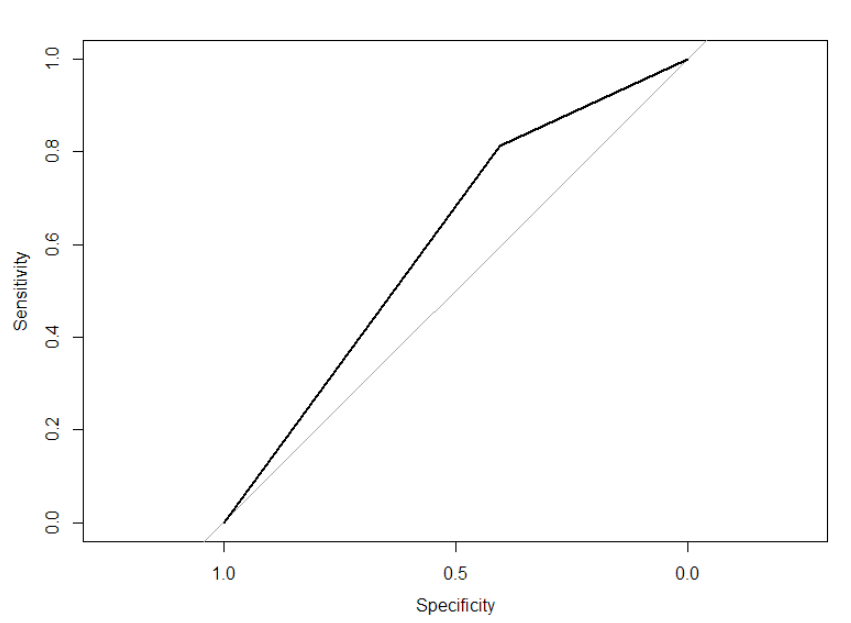
\includegraphics[scale=0.6]{images/06_roc.png}
	\caption[Grafico della ROC curve]{Grafico della ROC curve}
	\label{fig:perf-roc}
\end{figure}

Dal grafico della ROC è quindi stato possibile calcolare l'\textit{area under curve}, che determina la bontà generale del modello di predizione. \\ Il valore dell'AUC è risultato pari a 0.6103608.




\clearpage



\section{Web Demo}
\label{sec:ui}

Al fine di dimostrare l'utilizzo della rete in un applicativo software, viene qui illustrato lo sviluppo e il funzionamento di un'applicazione web che permette la configurazione delle rose dei due team coinvolti in una partita e la conseguente predizione del vincitore. Un ulteriore interfaccia permette anche la visualizzazione della Rete Bayesiana su cui effettuare inferenze specificando le variabili della query che si vuole sottoporre al modello Bayesiano.



\subsection{Architettura}

L'interfaccia web è stata sviluppata utilizzando l'architettura a 3 layer, con separazione di frontend, backend e database.

Il database utilizzato in fase di lettura è quello fornito inizialmente, senza alcuna modifica. Esso consiste quindi in un file SQLite interrogabile e modificabile semplicemente tramite un web server. Questo risulta particolarmente utile per fornire i dettagli dei giocatori ed eventualmente dei team così che l'utente possa visualizzarli e sceglierli attraverso l'opportuna interfaccia.

Per lo sviluppo del backend è stato deciso di utilizzare l'engine Javascript tramite il popolare progetto Node.js \cite{site:nodejs}. Esso è in grado di agire come middleware tra il frontend e il database, separando al meglio le logiche di manipolazione del dato. \'E inoltre incaricato di chiamare adeguatamente lo script R per la predizione del vincitore della partita e per svolgere le inferenze richieste.

Il frontend è invece sviluppato utilizzando la libreria Javascript React.js \cite{site:react}



\subsection{Interfaccia grafica}

Di seguito vengono mostrate brevemente le principali schermate dell'applicazione e il loro funzionamento.

All'avvio dell'app, utilizzando semplicemente un browser web, è possibile notare la schermata principale con 3 tab di selezione: {\it Home team}, {\it Away team} e {\it Results}. Mentre i primi 2 permettono di modificare le squadre, il terzo consente invece di visualizzare i risultati data la configurazione precedente.

% TODO : immagine

La schermata di configurazione della squadra mostra sulla sinistra l'immagine di un campo da calcio su cui è possibile spostare i giocatori, semplicemente trascinandoli col mouse e opportunamente aggiunti tramite il pulsante sulla destra, creando così la formazione da utilizzare.

% TODO : immagine

Una volta finita la configurazione cliccando sul tab dei risultati è possibile vedere in verde la squadra vincitrice e in rosso quella che invece è stata sconfitta.

% TODO : immagine

Per non dover ricreare configurazioni dall'inizio ogni qualvolta si avvii l'applicazione inoltre, nella parte superiore destra dello schermo sono presenti dei tasti per salvare e caricarne di precedenti.

% TODO : immagine



\subsection{Predizione risultato}

Per predire il vincitore della partita, come mostrato precedentemente, è stato necessario utilizzare la rete Bayesiana ottenuta a seguito degli esperimenti. Tale rete è stata infatti salvata su un file che è stato possibile poi ricaricare nell'ambiente R tramite l'apposito comando. Il web server javascript è dunque in grado di chiamare lo script R da riga di comando fornendogli in input una rappresentazione in formato JSON dei giocatori in campo con le loro caratteristiche. Lo script non deve far altro che manipolare i dati che gli sono stati forniti e applicare l'inferenza.

Per mostrare inoltre il puro funzionamento della rete è stato sviluppato un semplice form che permette l'inserimento delle evidenze e fornisce in output la probabilità che un certo evento si verifichi, coerentemente a quanto specificato dall'utente.



\clearpage



\section{Conclusioni}

Lorem ipsum dolor sit amet.




\newpage
\bibliographystyle{plainurl}
\bibliography{biblist}
	
\end{document}
